\documentclass{article}

\usepackage[a4paper, total={15cm, 24.5cm}]{geometry}
\usepackage{amsmath}
\usepackage{MnSymbol}
\usepackage{wasysym}
\usepackage{float}
\usepackage{graphicx}
\title{Formal Methods}
\author{Elia Ravella}
\begin{document}
	\begin{titlepage}
		\maketitle
	\end{titlepage}
	
	\tableofcontents
	\clearpage
	
	\part{Model Checking}
		\section{Requirements, Specification, Model Checking}
			We can represent a system and the environment surrounding it with a set of specifications and a set of requirements; these can be modeled as logical proposition (like FOL propositions). The model checking procedure is the formal technique to verify that certain properties holds, given the specifications.
		
		\section{Transition Systems}
			Transition systems are kinda like state automata, but they can be infinite (both in states and transitions), they do not have final states, and are modeled as
			\begin{equation}
				\langle S, Act, \rightarrow, I, AP, L \rangle = 
				\begin{cases}
					S \text{ the set of states}\\
					Act \text{ set of \emph{Actions}}\\
					\rightarrow \text{ transition relation: subset of } S \times Act \times S\\
					I \text{ subset of S, initial states}\\
					AP \text{ Atomic Propositions set, used as state labels}\\
					L \text{ labeling function } S \rightarrow 2^{AP}\\
				\end{cases}
			\end{equation}
			From a computational power point of view, transition systems are like finite state automata, and are usually called finite state machines as well\\
			From a suitability perspective, transition systems are perfect to model concurrent systems. Their representation is super similar to the FSA one:
			\begin{figure}[H]
				\centering
				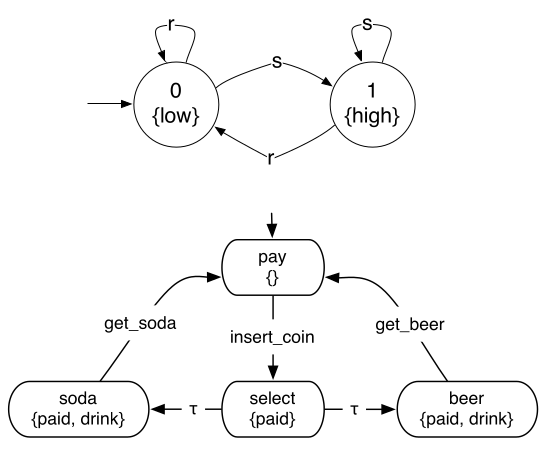
\includegraphics[width = \textwidth]{./images/TrSys.png}
			\end{figure}
			But transition systems supports \emph{variables} and \emph{conditional arcs}. These charts are usually called Program Graphs. States represent states and arcs represents instuctions (and can perform them). States are called \emph{locations} in this model. 
			
			\subsection{Linear Time Properties}
				With \emph{linear time property} is intended a desired behaviour of a system. A property of this kind (usually referred to as LT property) can be expressed in various forms, ranging from a ambiguous phrase "the system should behave like this" to a strict mathematical formulation.\\
				Formally, a LT property is a subset of $(2^{AP})^{\omega}$, which is the power set (set of all possible finite and infinite strings) of the transfer system. So, a LT property states "which \emph{traces} are valid" out of all possible traces the transfer system can generate.
				
			\subsection{Linear Time Properties Classification}
				\subsubsection{Safety Properties}
					Safety properties ensures that "bad things" don't happen. With "bad thing" is intended an illegal set of states, that corresponds to an illegal \emph{trace}.\\
					More formally, a safety property P over AP is a set of infinite words that \emph{all do not contain a bad prefix}, so a prefix where the illegal sequence appear.\\
					Even more formally,
					\begin{equation}
						P_{safe} \subseteq (2^{AP})^{\omega} \Rightarrow \forall \sigma \in (2^{AP})^{\omega} \backslash P_{safe} \,\vert\, \sigma' \notin \sigma
					\end{equation}
					Where $\sigma'$ is a bad prefix. An interesting property of safety properties (ahah) is $closure(P) = P$.
					
				\subsubsection{Invariants}
					Formal definition for invariant: a Linear Time property P over a set of atomic proposition AP is an \emph{invariant} if there is a logic formula $\phi$ so that \emph{all atomic propositions in P's traces satisfy $\phi$}.\\
					Checking if a property is an invariant is easy: it's enough to scan for a possible \emph{reachable} state that violates $\phi$.\\
					Wikipedia states that invariants are "a type of safety property in which the condition only refers to the current state".
					
				\subsubsection{Liveness Properties}
					A liveness property is a kind of LTP that \emph{does not rule out any prefix}. So what does this properties state? This kind of properties are "infinite words" properties such as starvation, that cannot be decided on a finite string. Where safety properties state "something bad don't happen", liveness properties state "something good eventually happens". \emph{They can be violated only in infinite traces}.\\
					Going full-formal:
					\begin{equation}
						\text{LT property } P_{live} \text{ is a liveness property if } prefix(P_{live}) = (2^{AP})^{\ast}
					\end{equation}
					
				\subsubsection{Fairness Properties}
					Fairness properties are even more abstract than liveness properties, and models the "common sense" behaviour of a system. In a traffic light scenario, we can model the interleaving of the lights as a liveness + safety property, but the fact the a traffic light becomes green infinitely often is not included in such set of properties. In practice, these properties rules out from the possible traces the ones considered \emph{not plausible} or \emph{not practically actuable, realistic}.\\
					They can be 
					\begin{enumerate}
						\item Unconditional: "Every process executes an arbitrary transition infinitely often". This property embodies the \emph{impartiality} property: for example, it describes the condition "a process enters its critical section infinitely often".
						\item Strong: "Every process that's ready to execute infinitely often executes an arbitrary transition infinitely often". This property is also called \emph{compassion}: its meaning is "if an activity is enabled it is executed infinitely often in the time period its enabled".
						\item Weak: "Every process that's ready to execute infinitely often from a certain time on fires a transition infinitely often". This is the \emph{justice} property: a process is infinitely often enabled \emph{\textbf{thus}} it's infinitely often executed.
					\end{enumerate}
					It also holds that $UF \Rightarrow SF \Rightarrow WF$. 
					
					
				\subsubsection{Safety vs Liveness}
					Relation between Safety and Liveness properties:
					\begin{enumerate}
						\item The \emph{only} property that's both a Liveness and a Safety property is $(2^{AP})^{\omega}$
						\item $LP \neq P_{live} \cup P_{safe}$, so there exist properties that are not safety nor liveness properties.
						\item $\forall P \in (2^{AP})^{\omega} \,\exists\, P_{safe}, P_{live} \,\vert\, P = P_{safe} \cap P_{live}$, or \emph{every property can be stated as a combination of a live and a safety properties on the same set of atomic porposition} (decomposition problem).
					\end{enumerate}
					
			\subsection{Equivalence}
				For transition systems exists am "equivalence" concept that makes use of the trace object: two transition systems are \emph{trace equivalent} with respect to some proposition if they produce the same trace with them. If two transition systems are equivalent they satisy the \emph{same} LT properties. This implies that two state if two transition systems are not equivelant it's enough to find a linear time property that \emph{is not} respected by one of them, but it s by the other

		\section{Model Checking Properties}
			\subsection{Model Checking Safety Properties}
				The model checking problem boils down to deduce if $TS \models P_{safe}$, so verify logically if the system (modeled as a transition system) is safe. The standard procedure consists of building an automata that recognizes the minimal bad prefixes in the model. The idea is to make the automata generate \emph{all} the bad prefixes in order to achieve
				\begin{equation}
					Trace(TS) \cap \mathcal(L)(autom) = \emptyset
				\end{equation}
				Another approach is to build a transition system that model the desired scenario, then check if the desired $P_{safe}$ can be derived by that. In practice, verify if:
				\begin{equation}
					TS \models P_{safe}
				\end{equation}
				or, equivalently:
				\begin{equation}
					TS \otimes \mathcal(L)(autom) \models P_{inv(\mathcal(A))}
				\end{equation}
				That means that the product of the transition system and the automata that recognizes the bad prefixes \emph{models} the "invariant safety property" that reduces the check to every single state. This last method is called reduction to invariant checking.
				\begin{figure}[H]
					\centering
					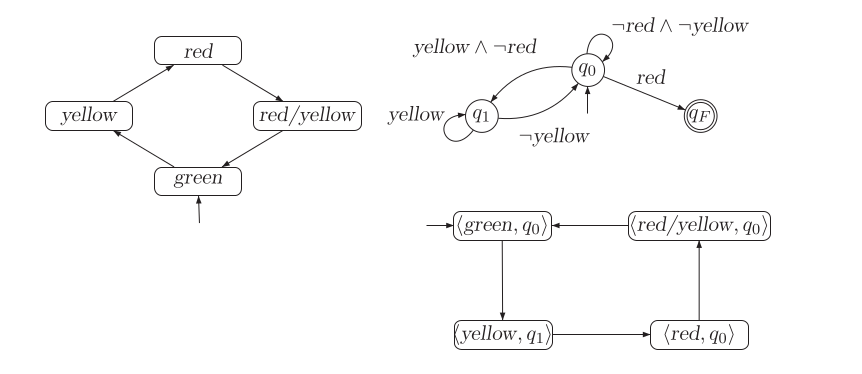
\includegraphics[width = \textwidth]{./images/TSProduct.png}
					\caption{Product of a transition system and an automaton modeling the safety property}
				\end{figure}
				
			\subsection{Model Checking Liveness Properties}
				The problem for liveness properties is their infinitiveness. The method is practically the same: we build a Buechi automata (an automata on infinite words), that's defined as a finite state machine but with multiple accepting states (the \emph{acceptance set}) and a different formulation for acceptance, that enables the recognition of infinite words: a never-ending word is accepted by a Buechi automaton if a state in the acceptance set can be reached infinitely many times while reading the input. For instance
				\begin{figure}[H]
					\centering
					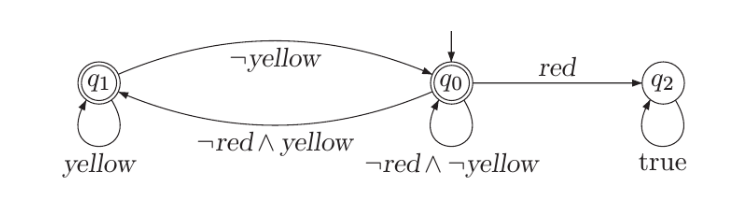
\includegraphics[width = \textwidth]{./images/NBA.png}
				\end{figure}
				is a nondeterministic Buechi automaton that checks the liveness property "red should be preceded by yellow". A pure liveness property "eventually forever $a$" can be verified by the automaton
				\begin{figure}[H]
					\centering
					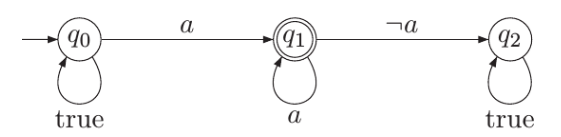
\includegraphics[width = \textwidth]{./images/NBA2.png}
				\end{figure}
				We then build the product of the TS and the Buechi automaton and we graph-check to verify that a path of the product infinitely often pass through an acceptance state (remember! acceptance state of a \emph{model checking Buechi automaton} represents the states that violate the property stated, as it model its complement) and show this path (if it exists) as a counterexample. If no such path is to be found, then the model satisfies the property by
				\begin{equation}
					Trace(TS) \cap \mathcal{L}_{\omega}(autom) = \emptyset
				\end{equation}
				Where $\mathcal{L}_{\omega}$ is the (language accepted by the) Buechi automaton, $\omega$ just stands for the infite lenght of the words considered.
		
		\section{Linear Temporal Logic}
			\subsection{Semantics}
				LTL is a propositional type of logic with a reduced set of operators, modified to match a sort of "automata like" transitions.
				\begin{equation}
					\phi = true \,\vert\, a \,\vert\, \phi \wedge \phi \,\vert\, \lnot \phi \,\vert\, \circ \phi \,\vert\, \phi \cup \phi \,\vert\, \diamond \phi \,\vert\, \square \phi 
				\end{equation}
				That represents
				\begin{enumerate}
					\item a thautology
					\item a proposition (so a \emph{state})
					\item composition
					\item negation
					\item next state. This operator is the "next time" operator in discrete time scenarios: $\circ^{k}$ is "true in $k$ instants"
					\item union, until
					\item eventually (somewhere in the future) (derived from the until operator)
					\item always (from now on forever) (derived from the until operator)
				\end{enumerate}
				
				\subsubsection{Past Operators}
					We can define the symmetric operator to the "next state", "eventually" and "always", respectively:
					\begin{itemize}
						\item yesterday: $\bullet \phi$
						\item sometimes in the past: $\blacklozenge \phi$
						\item always in the past: $\blacksquare \phi$
					\end{itemize}
					The introduction of past operators enhances the readability of the formulae, but \emph{does not enhance the expressivity of LTL}.\\
					The combination of "always in the past" and "from now on forever" is the $Alw = \square \phi \wedge \blacksquare \phi$ operator.
				
				\subsubsection{Metric of Time}
					Two operators ($\mathcal{U} \text{ntil and } \mathcal{S} \text{ince }$) are usually introduced when the time concept is introduced. They also can be derived from the "tomorrow" and "yesterday" operators, but again they simplify a lot the formulae.
		
			\subsection{Fairness in LTL}
				\begin{itemize}
					\item Unconditional fairness: $\square \diamond \psi$
					\item Strong fairness: $\square \diamond \psi \Rightarrow \square \diamond \phi$
					\item Weak fairness: $\diamond \square \psi \Rightarrow \square \diamond \phi$
				\end{itemize}
				
			\subsection{LTL Model Checking}
				It's easier to write down a property in form of LTL property instead of a Buechi automaton. This makes the model checking procedure on LTL models faster and more intuitive. Anyway, the construction of a Buechi automata is involved in the checking of a LTL model.
				
				\paragraph{Positive Normal Form}
					We need a LTL definition that's "easy to invert". The PNF helps us: in a PSF formulated proposition, the negation only appears adjacent to atomic proposition. This helps because such a formula is easy to invert. We must add to LTL the operator "Weak Until", defined as:
					\begin{equation}
						\phi \,W\, \psi = (\phi \cup \psi) \vee \square \phi
					\end{equation}
					This operator aid the "transporting" of the negations inside and out the union / until operator.\\
					Another useful operator is the Release Operator:
					\begin{equation}
						\phi \,R\, \psi = \lnot(\lnot \phi \cup \lnot \psi)
					\end{equation}
					
				\subsubsection{Automata Based LTL Model Checking}
					We build a Buechi automaton that only accepts the negation of our LTL model. Not a simple Buechi automata, but a generalized one, in which a set of acceptance states is repeated infinitely often. Then, we transform the GBA in a NBA with the property previously stated.\\
					BUT WAIT: a NBA derived from a LTL formula $\phi$ has at least $2^{\vert \phi \vert}$ states. That's a LOT.
					
				\subsubsection{Bounded Model Checking}
					We want to verify properties \emph{without using a Buechi automaton}. Instead, we want to use the SAT formulation. The "bounded" refers to the fact that \emph{to find a counterexample} you only need to traverse paths of bounded lenght (for the product of a TS and a property thins number is number of states + 1).\\
					To do so, we translate the condition "unfolding up to k steps" to a boolean formula and it's satisfied if \emph{a counterexample is found}.\\
					Remember! This procedure, in some way, is just \emph{encoding in a binary system} all the possible state (they're represented as a \emph{set of conditions}, so a \emph{set of true/false statements}) and then translating the Transition relation in a binary function that does the same.
					
					\paragraph{Unfolding}
						We can't stray a lot far from FSMs. We should find a way to translate the state transitions as boolean formula, and this is done by selecting a set of boolean variables (and their "twins" of the next state) that are then passed through a Transition function that describes the next state in terms of \emph{that very variables}. The \emph{unfolding} of the transition function generates a boolean model for all the bounded paths for the TS.
						
						\begin{figure}[H]
							\centering
							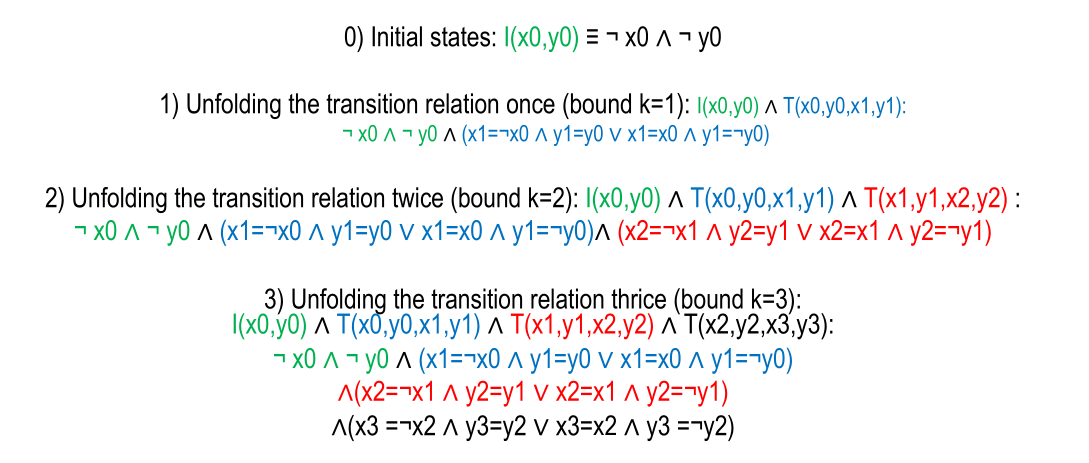
\includegraphics[width = \textwidth]{./images/unfolding.png}
							\caption{Unfolding of a 4 states automaton through its boolean transition function. Can be noticed that for each transition, the next state is described as a current state evolution.}
						\end{figure}
						
						The formal definition of the unfolding operation is:
						\begin{equation}
							\vert [M] \vert_{k} = I(S_0) \wedge ( \bigwedge_{0 \leq i < k}T(S_{i}, S_{i + 1}) )
						\end{equation}
						Where $S_0$ is the initial state (described by means of the boolean variables) and $S_i$ represents the state of the automaton at the $i-th$ iteration of the unfolding procedure.
						
					\paragraph{Loops and Variables}
						Once the system is described in a boolean formula, we must add a loop condition (a loop represent problem for formulae, because it changes the "time flow" and the evolution of an unfolding) and a boolean definition of the \emph{negation} of the property we're trying to prove and SATcheck that formula.\\
						We also have to introduce "formula variables" that simply are the unfoldings of the system \emph{bounded in steps} and \emph{bounded logically} to respect a certain property. We will define our properties over these new variables (that now have a notion of evolving system) in order to check for a specific property.\\
						Last but not least, we have to redefine also the Until and Release operator to work with this new time formulation. Where's the problem? Problems arise when loops appear.
						
					\paragraph{Verifing}
						Now that we have a procedure to turn the evolution of a TS (or an automaton) into a boolean formula verifing it is easy: just build the logic formula up until instant $k$ and verify such formula. So:
						\begin{enumerate}
							\item Build $\vert [M] \vert_{k}$ unfolding of the transition relation up to instant $k$ that \emph{is a propositional formula}
							\item Insert loop variables to detect loops
							\item Build the LTL formulation of the property we're trying to verify over the formula variables of the system described in 1 and 2. We'll call this $\Phi$
							\item SATcheck $\Phi$
								\begin{itemize}
									\item If a counterexample is found, the property does not hold
									\item If a counterexample is not found, the property holds \emph{up to instant k}
								\end{itemize}
						\end{enumerate}
					
		\section{Cuncurrency Constructs - Parallel Compositions}
			\subsection{Interleaving}
				Interleaving is one of the most simple cuncurrency model: two activities (processes) alternate their usage of the CPU without synchronizing. The interleaved operator is $\vert \vert \vert$. The interleaving between two transiction systems is defined as:
				\begin{equation}
					TS1 \,\vert\vert\vert\, TS2 = \langle S_1 \times S_2, Act_1 \cup Act_2, \rightarrow, I_1 \times I_2, AP_1 \cup AP_2, L \rangle
				\end{equation}
				As can be seen, the total number of states id $\vert S_1 \vert \times \vert S_2 \vert$. The transiction function "$\rightarrow$" is modified this way:
				\begin{equation}
					\text{transiction } s_1 \xrightarrow{\alpha} s_1' \text{ becomes } \langle s_1, s_2 \rangle \xrightarrow{\alpha} \langle s_1', s_2 \rangle 
				\end{equation}
				So at any transiction only one machine is considered active.\\
				Interleaving causes problems when the two processes share variables. The two executions can overwrite each other's value on those shared variables or read incnsistent ones. Obviously this causes faults.\\
				
			\subsection{Handshaking}
				Handshaking introduces "synch actions" that makes parallel computations synchronize. $TS_1 \,\vert\vert\,_{H} TS_2$ means that the two computations uses actions in the set $H = \subseteq Act_1 \cap Act_2$. The two transitions evolve indipendently (so interleaving) on other events. This handshake is a "Petri net"ish one. Obviously, if $H = \emptyset$, handshaking boils down to interleaving.\\
				The transformation of rules is similar to the interleaved one; the only difference appears when the read symbol (the action) is part of the H set. In that case, \emph{both} states changes. Formally
				\begin{gather}
					s_1 \xrightarrow{\alpha} s_2 \\
					t_1 \xrightarrow{\alpha} t_2 \\
					\text{becomes } \langle s_1, t_1 \rangle \xrightarrow{\alpha} \langle s_2, t_2 \rangle
				\end{gather}
				if $\alpha$ is in set H.\\
				An example (that only shows the three machines and the handshake actions are labeled in the same way) is the "passaggio a livello" one. 
				\begin{figure}[H]
					\centering
					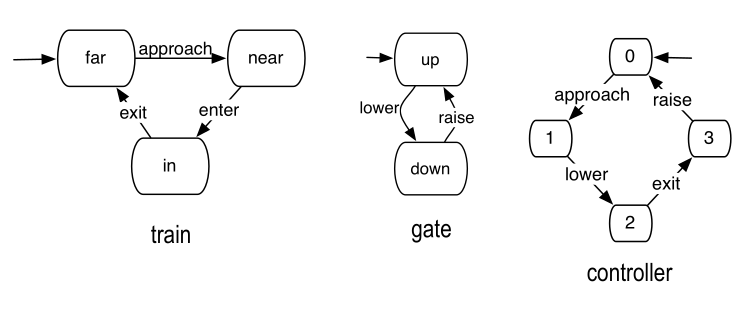
\includegraphics[width = \textwidth]{./images/PAL.png}
				\end{figure}
					
			\subsection{Channel Compositions}
				Channels adds directionality to handshaking compositions. Transiction systems can model FIFO channel (like a networking idea one) by interpreting each move of the machine as a send*receive action, signaled by the last character. For example
				\begin{figure}[H]
					\centering
					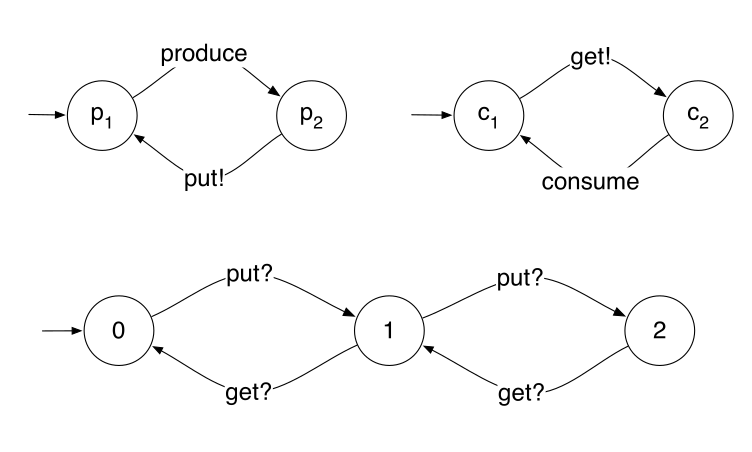
\includegraphics[width = \textwidth]{./images/Channels.png}
					\caption{A produce-consume system. Notice how this is just a directional handashaking. Why? See below, capacity.}
				\end{figure}
				For a channel, we call capacity the maximum number of events it can store. If capacity is equal to zero channels implements handshaking through \emph{synchronous message passing}.\\
				Asynchronicity is possible (capactiy $\geq$ 1 and not fulled) \emph{but} a read action is possible only if it's reading the token on top of the channel (for the FIFO propeerty). The formalism is "token!" for writing token on the channel and "token?" for reading token from the channel.
				
				\paragraph{Example of a modeling language with channel - Nano Promela Spin}
					Promela is a set of interleaving processes that can communicate through channels. The syntax of Spin (that is promela, reduced). is
					\begin{equation}
						statement = 
						\begin{cases}
							skip \text{ represents a process that terminates in one step, without side effects}\\
							x := expr \\
							c?x \\
							c\lnotexpr \\
							statement;statement \text{ sequential composition}\\
							atomic\{assignements\} \\
							if :: g1 \,\Rightarrow\, statement ... fi \\
							do :: g1 \,\Rightarrow\, statement ... od
						\end{cases}
					\end{equation}
					The if instruction has some peculiar properties. First of all, it's an Erlangish if, with a list of guards that can be satisfied or not. The choice of the right branch to take is \emph{nondeterministic}. The if is a blocking operation if no guard is satisfied. Also, testing the guard and executing the body is an \emph{atomic} operation. The same properties are shared by the loop construct "do :: od". The loop continues until one guard is true.\\
					Useful example, the good ol' vending machine:
					\begin{figure}[H]
						\centering
						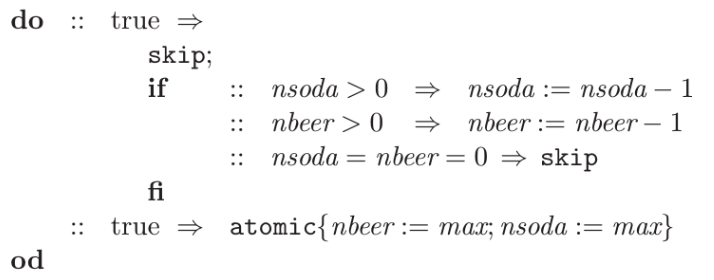
\includegraphics[width = \textwidth]{./images/VendingSpin.png}
					\end{figure}
					What to notice: 
					\begin{itemize}
						\item the refilling is modeled as atomic because we want to prevent people buying stuff while we refill the machin
						\item at each iteration nondeterminstically is chosen either to block the program on a vending operation or to refill the machine if there are no more cans
					\end{itemize}
					Programs in this language can be expressed in program graphs:
					\begin{figure}[H]
						\centering
						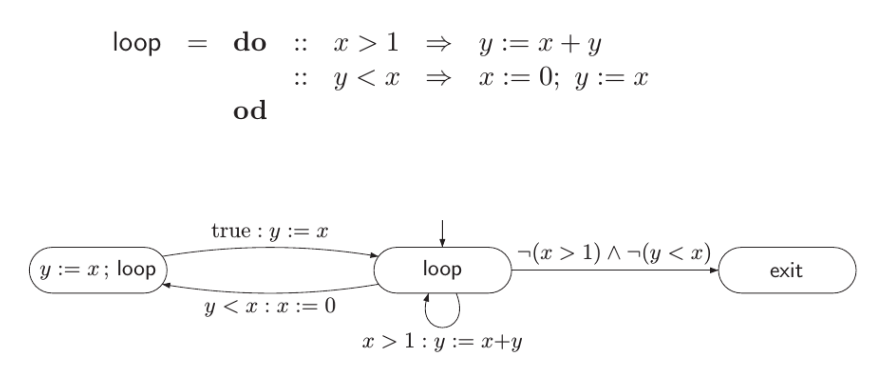
\includegraphics[width = \textwidth]{./images/PromelaGraph.png}
					\end{figure}
					
					
		\section{Abstraction and Refinement}
			Abstraction is the procedure of getting further from the actual reality of a model in order to maintain only the properties of interest. Refinement is the opposite: adding details to a model to make it more adherent to the original system (so, augmenting complexity).\\
			To abstract and to refine a transition system (or a more general system of sort) can be viewed as a procedure that scans equivalent systems with the purpose of verifying property that are hard to verify in the original, most refined, max complex real system. To do so we need a concept of equivalence (or at least of order, borrowing from logic) between transition systems. We can use two approaches, one that takes into consideration the property of the states of a TS and one that instead checks for equivalence in the traces of a TS. Depending on the type of property we want preserved, we can apply a different kind of equivalence or order. 
					
			\subsection{Bisimulation}
				We introduce the \emph{Bisimulation Equivalence} this way:\\
				A bisimulation $TS_1 \sim TS_2$ is a binary relation $\mathcal{R} \subseteq S_1 \times S_2$ so that
				\begin{equation}
					\forall s_1 \in I_1 (\exists s_2 \in I_2 \,\vert\, (s_1, s_2) \in \mathcal{R}) \text{ and viceversa}
				\end{equation}
				and also, for all $(s_1, s_2) \in \mathcal{R}$
			 	\begin{enumerate}
			 		\item states are equivalent if they've got the same label
			 		\item final states must be equivalent
			 		\item the "match" property: $\forall s_2' \in Post(s_2) \exists s_1' \in Post(s_1) \,\wedge\, (s_2', s_1') \in \mathcal{R}$ and viceversa. This is the "match every move" property.
			 	\end{enumerate}
			 	The idea behind the bisimulation relation is to introduce formally a way to "make a machine simulate another" by matching every transition of the first with every transition of the second.\\
			 	A bisimulation relation is reflexive, transitive and symmetric $\Rightarrow$ it's an equivalence relation.
			 	
		 	\subsection{Simulation Relation}
		 		A simulation relation is an asymmetric bisimulation (wrong but intuitive definition): "a system can simulate another \emph{but not vice versa}". Simulation relation are useful in an abstraction procedure, and generally is easier to prove simulation in one way than in both.\\
		 		The formal definition of the Simulation relation is \emph{exactly the same} of the bisimilation one, it just lacks the reflexivity constraints.\\
		 		It is: TS2 simulates TS1 ($TS2 \succeq TS1$) if and only if
		 		\begin{equation}
					\forall s_1 \in I_1 (\exists s_2 \in I_2 \,\vert\, (s_1, s_2) \in \mathcal{R})
				\end{equation}
				and forall ($s_1, s_2$) in $\mathcal{R}$ it holds that
				\begin{enumerate}
					\item $L(s_1) = L(s_2)$
					\item $s'_1 \in Post(s_1) \Rightarrow \,\vert\, \exists s'_2 \in Post(s_2) \,\vert\, (s'_1, s'_2) \in \mathcal{R}$
				\end{enumerate}
		 		The simulation relation is an \emph{order} relation.
		 		
	 		\subsection{Simulation Equivalence}
	 			It can be possible that $TS2 \preceq TS1 \,\wedge\, TS1 \preceq TS2$, so the two system can simulate each other. This condition is called \emph{simulation equivalence}, and it pops up when there's a symmetric portion of the simulation relation. It's usually expressed as $TS1 \simeq TS2$.\\
	 			\textbf{\emph{THIS IS NOT A BISIMULATION}}.\\
	 			Although being not a bisimulation, two simulation-equivalent systems satisfy the same \emph{safety} properties.
			
			\subsection{Trace Inclusion}
				First, we need to formalize the concept of "making a system mor refined". To do so we introduce the Implementation relation, or Trace Inclusion, stated as:
				\begin{equation}
					Trace(TS1) \subseteq Trace(TS2) \,\Leftrightarrow\, TS1 \text{ is an implementation of } TS2
				\end{equation}
				the idea is quite simple: not all abstract scenarios are contemplated by the real system. Again, the inclusion relation is an order relation on traces (not anymore on states).
				
			\subsection{Trace Equivalence}
				As we did for Simulation and Simulation Equivalence, we do for Trace Inclusion and Trace Equivalence: this time is easier, we just use the "trace equivalence" concept explained in 2.3.
				
			\subsection{Relation Between Equivalences}
				Bisimulation is the largest equivalence relation on the TS set. It implies Trace Equivalence and Simulation Equivalence, that each implies the order relation from which it has been derived. To sum up this relations, we can use the schema
				\begin{figure}[H]
					\centering
					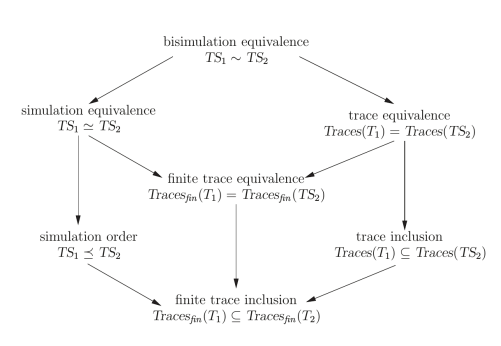
\includegraphics[width = \textwidth]{./images/Relations.png}
				\end{figure}
				A few notes on the schema:
				\begin{itemize}
					\item The "finite trace equivalence" and "finite trace inclusion" binary relations are peculiar, beacuse they "bridge the gap" between a relation on states (the simulation) and one on traces (trace equivalence). This is achieved by adding the constraint (to the simulation relation) that the TSs are non terminating (no final states). This is due to the fact that the presence of final states conditions the shape of the traces, and in the simulation relation traces are ignored; this could lead to states in the simulating machine that are simulating both a final and nonfinal state of the simulated machine\footnote{In practice, it's not difficult to model a system as nonterminating, especially a cuncurrent or real time one.}.
					\item Safety properties are preserved by simulation: (always with the no-final-states assumption) $(TS1 \preceq TS2 \wedge TS2 \models P_{safe}) \Rightarrow TS1 \models P_{safe} $
					\item Given the above distinction, we can link simulation relation and trace equivalence! In fact, if we consider two TSs with no terminal states, $TS1 \preceq TS2 \Rightarrow Trace(TS1) \subseteq Trace(TS2)$
						\begin{itemize}
							\item Corollary: \emph{for transition systems without final states}, all LT properties (not just safety ones) are preserved by the simulation relation.
						\end{itemize}
				\end{itemize}
			
			\subsection{Abstraction, Refinement, Simulations}
				The quite abstract concepts of Abstraction and Refinement can be expressed via the simulation relation. In fact, we can say that
				\begin{equation}
					TS1 \text{ is a refinement of } TS2 \Rightarrow TS1 \text{ is simulated by } TS2
				\end{equation}
				and vice versa for abstraction:
				\begin{equation}
					TS1 \text{ is a abstraction of } TS2 \Rightarrow TS1 \text{ simulates } TS2
				\end{equation}
				To sum up the reasoning, \textbf{a more abstract system simulates a refined one} (if it has been obtained from it).
	
			\subsection{Relations with Actions}
				So far, the only criterion used to distinguish two states was the one-step-reachable states and the labels. What about actions? Actions are usually ignored in model checking, where usually "labels of transitions" are considered irrelevant. Nonetheless, we can redefine all the seen binary relations between TSs to take into consideration actions:
				
				\paragraph{Action Based Bisimulation}
					The action-based bisimulation is formalized as: let TS1 and TS2 transition system over the same Act set, they are action-based bisimilar if and only if
					\begin{enumerate}
						\item $\forall s_1 \in I_1 (\exists s_2 \in I_2 \,\vert\, (s_1, s_2) \in \mathcal{R}) \text{ and viceversa}$
						\item $(s_1 \,\xrightarrow{\alpha}\, s'_1) \,\Rightarrow\, s_2 \,\xrightarrow{\alpha}\, s'_2 \wedge (s'_1, s'_2) \in \mathcal{R} \text{ and viceversa}$
					\end{enumerate}
					TS1 is action-bisimilar to TS2 is expressed as $TS1 \sim^{Act} TS2$.\\
					The action-based bisimulation relation is finer than the state-based one, but it can be straightforwardly adapted.
			
			\subsection{Remark, Abstraction Function}
				An important phase of the abstraction procedure is to decide \emph{which detail to omit in the abstraction}. This is usually formalized by means of an abstraction function, so a function from the "refined" domain to the "abstract" domain of states. This function just links each refined state to the corresponding abstract state. By definition, this is usually a non-injective function, as it tends to "group" refined states into more meaningful abstract states.
				
			\subsection{Further: Stuttering Equivalence}
				Equivalence as seen so far is described "state by state". The stuttering equivalence, instead of matching step by step evolutions of a TS, matches \emph{path fragments}: single transitions can be mapped to paths.
				
				\subsubsection{Stutter Bisimulation}
					Formal definition for a stuttering bisimulation:\\
					Let TS be a transition system. A stutter bisimulaton for TS (denoted as $\approx_{TS}$) is a binary relation on $\mathcal{S} \times \mathcal{S}$ so that
					\begin{enumerate}
						\item $L(s_1) = L(s_2)$
						\item $ (s'_1 \in Post(s_1) \,\wedge\, (s'_1, s_2) \notin \mathcal{R}) \,\Rightarrow\, (\exists s_2 u_1 ... u_n s'_2 \,\wedge\, n \geq 0 \,\wedge\, (s_1, u_i) \in \mathcal{R} \forall i \leq n \,\wedge\, (s'_1, s'_2) \in \mathcal{R})$ and viceversa
					\end{enumerate}
					
		\section{Symbolic Model Checking}
			\subsection{Branching Time Logics}
				BTL is based on the assumption that time itself can be represented as a tree, where each istant has multiple futures. It's a useful tool when properties like "it's possible that" etc. Computation Tree Logic is the simplest BTL we can define.
				
				\subsubsection{Computation Tree Logic}
					Given a transition system, we can derive the computation tree by just unrolling all the computations that are possible. It's kinda a reachability tree. If the transition system allows loops, the computation tree is infinite in height. Computation trees are useful when an analisys on execution is to be made, because thy're easier to handle that simple traces.
			
				\subsubsection{LTL and computation trees}
					Most of the LTL formulaes can be expressed to work on computational trees, but not all of them: due to the very logic-like expression of the LTL formulaes, they cannot model properties like "of all possible executions, \emph{at least one} gives the output $x$".
				
			\subsection{Syntax for CTL}
				CTL supports two kinds of formulae, one for the current state and one for the paths.
						
				\subsubsection{State Formulae}
					Classic logic formulae. They express properties of the single state and the branching structure. The two "new" operators here are $E\,\phi$ and $A\,\phi$ that express "exists a path exiting from this moment where $\phi$ holds" and "forall paths etc."\\
					The formal definition is so:
					\begin{equation}
						\Phi ::= true \,\vert\, a \,\vert\, !\Phi \,\vert\, \Phi_1 \,\wedge\, \Phi_2 \,\vert\, E\varphi \,\vert\, A\varphi 
					\end{equation}
					where $\Phi$ is a valid formula, $a$ is a propositional letter and $\varphi$ is a path formula.
					
				\subsubsection{Path Formulae}
					Path formulae express temporal properties of paths. \emph{They cannot be linked with boolean operators}, but they support Until and Next-Step operators. The path formulae express properties that must hold for all states in the path.\\
					Again, the formal definition is
					\begin{equation}
						\varphi ::= X \Phi \,\vert\, \Phi_1 \mathcal{U} \Phi_2
					\end{equation}
					Where $\Phi$ is the state formula. Notice how two path formulae can be connected only through E and A operators ($\varphi$ alone is not a valid formula). Also, notice how this implies that a formula like $FG a$ is never a valid formula in CTL, because there's no quantifier.
					
				\subsubsection{CTL Patterns}
					CTL can be very hard to understand, so a set of shorthands and pre-cooked patterns can be defined and used as building blocks instead of pure raw logic operators.\\
					There are additional state operators as:
					\begin{itemize}
						\item X: next state (so $X\Phi$ stands for "in the next state, $\Phi$ holds"
						\item F: eventually, on this path, $\Phi$ is verified
						\item G: "forever on this path"
					\end{itemize}
					
					These are the most common combinations of path-state operators:
					\begin{itemize}
						\item $EF\Phi = E(true \,\mathcal{U}\, \Phi)$ that states that at least one path from now on has only $\Phi$ after some point
						\item $AF\Phi = A(true \,\\matchal{U}\, \Phi)$ all paths, eventually
						\item $EG\Phi = !AF(!\Phi)$, or "exists a path of all $\Phi$" from now on 
						\item $AG\Phi = !EF(!\Phi)$, or "all path are all $\Phi$" from now on
					\end{itemize}
					
					Most common patterns:
					\begin{itemize}
						\item $AG(req \,\Rightarrow\, AF good)$ or "on all paths, any request is followed (also not immediately) by a state where \emph{good} holds". 
						\item $AG AF enabled$ that ensures that an \emph{enabled} state is eventually reached on all states.
						\item $AF AG good$ states that all path, eventually, will lead to a non terminating sequenco of \emph{good} states
						\item $AG EF restart$ "on all possible path a restart is always \emph{possible}". Note the concept of \emph{possible}, that's impossible to describe in standard LTL, is used pretty easily in this kind of fomrulae.
						\item $EF(started \,\wedge\, !ready)$ or "it is possible to reach a state where started holds, but not ready". 
					\end{itemize}
					
				\subsubsection{CTL vs LTL}
					A theorem proves that CTL and LTL are not comparable. This is because we cannot express in any way in LTL the \emph{E} operator of CTL. On the other hand, some LTL formulas (as $\diamond \square a$) cannot be reproduced in CTL because of the mechanics of the quantifier operators.\\
					There's a way to find if two formulae (one CTL and one LTL) are equivalent, and it is described in this theorem:
					\begin{equation}
						\Phi \in CTL, \varphi \in LTL \,\vert\, \varphi = \Phi \text{ without all path quantifiers} \Rightarrow
						\begin{cases}
							\Phi = \varphi\\
							\vee\\
							\text{no LTL formula is equivalent to } \Phi
						\end{cases}
					\end{equation}
					So either two formulae are easy to prove equivalent (removing the quantifiers and in case rewriting to some equivalent formulae) or there are no formulae that can express the same property.\\
					For instance: $AGAF \, a \equiv GF \, a$ but $AFAG \, a \nequiv FG \, a$ and also 
					\begin{itemize}
						\item no LTL formula can express AFAG
						\item no CTL formula can express FG
					\end{itemize}
					
				\subsubsection{Fair CTL}
					CTL cannot express fairness. To include fairness contraints inside a CTL properties specification, the tipical approach is to define the system over a set of paths \emph{that are already fair}. This is usually done by means of a LTL formula expressing the fairness constraint and then a CTL specification of the other properties.
					
				\subsubsection{CTL Equivalence}
					We can define a equivalence relation using the CT logic this way: two states are equivalent of they cannot be distinguished by any truth value of any formulae in the logic. The formal definition for CTL-equivalence (directly between systems, between states is the same) is:\\
					let TS1 and TS2 transition systems over the same AP and with no terminal states, so with only infinite traces. TS1 $\equiv_{CTL}$ TS2 if and only if
					\begin{equation}
						TS1 \models \Phi \wedge TS2 \models \Phi \forall \Phi \text{ over AP}
					\end{equation}
					A remarkable property of CTL equivalence is that for finite transition systems with no terminal states \emph{it corresponds to bisimulation}.
					
			\subsection{Symbolic MC}
				The step towards symbolic MC from CTL model checking is the same done by the BMC; the operations on states are replaced by \emph{set operations}, the transitions are grouped and handled as \emph{sets of transitions} as a whole.\\
				States and functions of a transition system must be encoded in binary, so we
				\begin{enumerate}
					\item Encode each state in a binary form ($n = $ number of states $\Rightarrow \vert encoding(S_i) \vert = \lceil \log_2(n) \rceil$, where $S_i$ is a state).
					\item Represent the transition relation as a \emph{binary boolean} relation
						\begin{equation}
							f_{\rightarrow} \,:\, \{0,1\}^n \,\times\, \{0,1\}^n \,\rightarrow\, \{0, 1\}
						\end{equation}
						This can be represented as a $n \times n$ matrix \emph{of only 1s and 0s}.
					\item Optimize the encoding of the $f_{\rightarrow}$ function with every method of the digital design course (Shannon expansions...). We'll focus on the optimization of the Ordered Binary Decision Diagram.
				\end{enumerate}
				
				\paragraph{Ordered Binary Decision Diagram}
					An OBDD is the binary expansion of a formula. At each level every variable in the formula is considered true for a subgraph and false for the other one. In the leaves there's the truth value of that specific combination. Example:
					\begin{figure}[H]
						\centering
						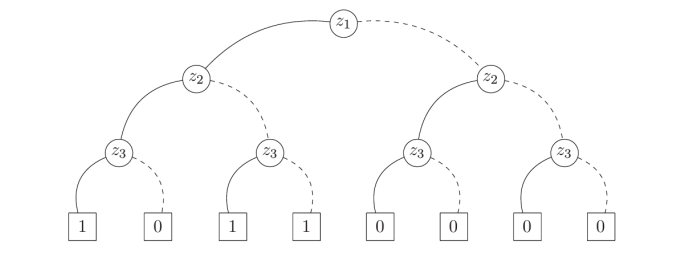
\includegraphics[width = \textwidth]{./images/OBDD.png}
						\caption{OBDD for the formula $z_1 \,\wedge\, (!z_2 \,\vee\, z_3)$}
					\end{figure}
					In this example, right subtrees consider the variable negative, left subtrees positive. Straightforwardly from the formula (and her OBDD representation) it can be noted that the value of some variables condition the overall truth value in a significative way: for example, $z_1 = false$ implies that the formula is false. This kind of relationships can help simplify the graph:
					\begin{figure}[H]
						\centering
						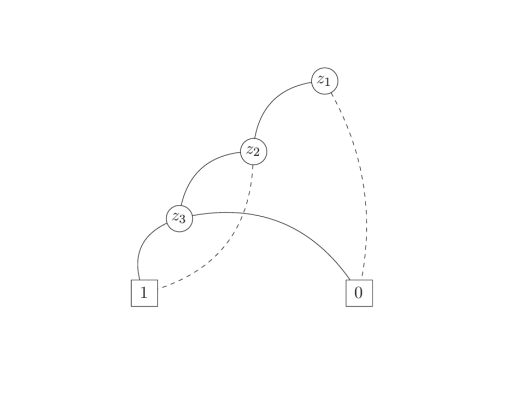
\includegraphics[width = \textwidth]{./images/OBDD2.png}
						\caption{Grouping together all the paths that lead to the same values.}
					\end{figure}
					Dashed lines represent "false" while straight lines "true".\\
					The OBDD optimization can result in great performance improvement of the overall algorithm: operations on the single states can result in "bigger" operation on the whole OBDD or result in no operation, having no effect on the whole system. 
					
		\section{Timed Automata}
			Even "timed LTL" (the version of LTL that takes care of the "steps" of the system) isn't enough to fully express a system (an asynchronous one) in detail \emph{when time is a crucial characteristic} (time sensitive - real time systems, security / safety systems). In FSM, time is assumed to be metric, implicit and discrete. In Buechi automata, it's also infinite.\\
			Time and timing issues start to creep out in the FSM field when we introduce parallel composition: can we preserve the "one transition = one time step" relation? And moreover, how can we introduce \emph{asynchronicity} to this model, given that parallel composition do not preserve timing relationships? There are several ways:
			\begin{itemize}
				\item Time advances only when \emph{certain} transitions are taken, or conditions met; this method is suitable for systems that must synchronize (so subsystem can "agree" on when to sync). This does not eliminate statecharts and transition dependency, tho.
				\item Transition-indipendent time flow: this is usually done by adding \emph{guards} on transitions that specifies \emph{when} a certain transition is taken (after how much time, at which time instant ecc). This model can capture the notion of continuous time, also. This approach gives timed and hybrid automata.
			\end{itemize}
			
			\paragraph{Formal Definition of a TA}
				A Timed Automaton is an automaton whose graph is augmented with some real values, called clocks. These values are associated to states: a state is a combination of a location (so its label, the \emph{logical state}) and a set of clocks. A TA evolves in two possible ways:
				\begin{itemize}
					\item Time passes (no state change)
					\item State change (time is stopped)
				\end{itemize}
				In this model, the clocks can be only inspected or reset. Each clock can be associated to an arc (on which it represents the period of time in which that transition can be fired) or to a state (where it signals the amount of time that can be spent in that state). State clock are often called \emph{invariants}.\\
				Example:
				\begin{figure}[H]
					\centering
					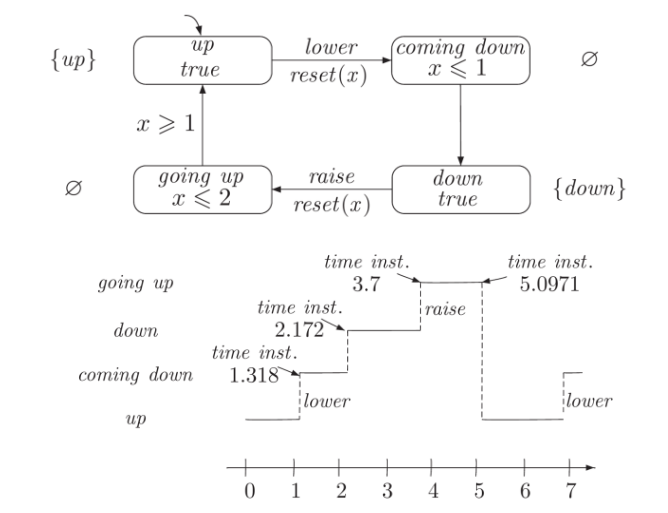
\includegraphics[width = \textwidth]{./images/TA1.png}
				\end{figure}
				Parallel composition can also be defined for timed automata: it's easy when we consider the labels of the arcs as the union of the label itself and the clock constraints; at that point, the composed label is the union of the label and the conjunction of the clock constraints. All the non-sync transitions (the interleaved one) are computed as usual (so, interleaved).\\
				As an example:
				\begin{figure}[H]
					\centering
					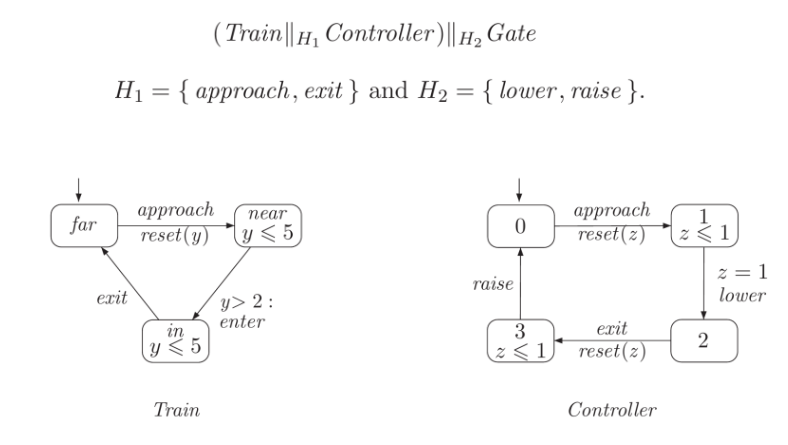
\includegraphics[width = \textwidth]{./images/TAex1.png}
					\caption{The two separate systems that describes the train and the controller. To be noted: the arc labeled the same way will be the one to synchronize on.}
				\end{figure}
				\begin{figure}[H]
					\centering
					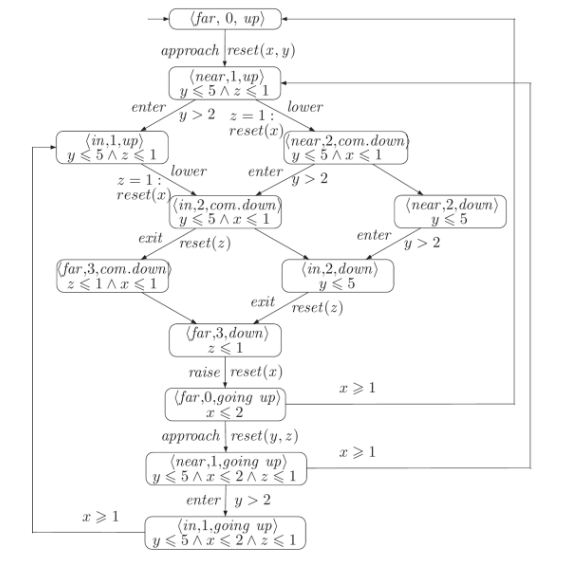
\includegraphics[width = \textwidth]{./images/TAex2.png}
					\caption{The resulting handshook TA with synchronized behaviours.}
				\end{figure}
				
			\paragraph{Time Problems}
				Introduction of time in automata conduces to two major possible problems: timelock and Zeno paths.
				
				\subparagraph{Timelock}
					A state contains a \emph{timelock} if there's no time-divergent path exiting from him. \emph{The time do not advance}, exiting from that state. For converging time we mean the serie that regulates the evolving of time converges.
					
				\subparagraph{Zeno Paths}
					A subpath is called a \emph{Zeno path} if it's infinite and time convergent (time do not progress) and also \emph{infinite many actions are executed along it}.
					
				\subparagraph{Likelihood of Time Problems}
					Both timelock and Zeno paths are considered very unlikely to show up; the former because of it's very difficult for time to completely stop (and the invariants are there for a reason) while the latter because the additional action-taking constraint will imply infinite computational power to enable them.
				
			\subsection{Clock Regions}
				If we put on a plane the time passing and the value of the clocks of the system (it will be a discrete plane) we can define an equivalence relation on clock values. In this case, our formal relation of equivalence renders equal two clock if their integer part is equal and the fractional part is "in order" (so two clock "agree" on the fractional order)  we can also define the equivalence sets for this equivalence and call them \emph{clock regions}. 
				
				\paragraph{Time Successor Relation}
					We need to define the successors of a clock region, quite easy: the successors for all the clock evaluations inside a clock region are the evaluation of all the clock with a finite offset. 
					
				\paragraph{Time Abstracted Bisimulation}
					Theorem: clock equivalence is a bisimulation equivalence over AP'. This enables us to build \emph{finite} automata \emph{which also preserve CTL formulae}.
				
		\section{Hoare Method}
			The Hoare's method model program through preconditions and postconditions of its functions. Hoare uses first order logic to do so, defining a $Pre(var)$ and a $Post(var)$ sets, where \emph{var} is the set of variables taken into consideration. The basic solving method is based on substitution: expressions that modify the values of variables \emph{specified in the conditions} is replace \emph{directly in the formula} in the place of the variable itself.
			
			\paragraph{Syntax and Logic Stuff}
				Keepeing in mind the substitution rule
				\begin{equation}
					\{Post_x^{exp} x := exp\{Post\}\}
				\end{equation}
				that allows us to \emph{verify the logic formulae}, we introduce the "deduce" structure
				\begin{equation}
					\frac{\{P\} \, S_1 \, \{R\}, \,\,\, \{R\} \, S_2 \, \{Q\}}{\{P\} S_1, S_2 \{Q\}}
				\end{equation}
				That simply means that the above formula is true, we can deduce the lower formula. With this notation, we can build up the basic programming languages features:
				\begin{equation}
					\frac{\{P \wedge c\} \, S_1 \, \{Q\}, \,\,\, \{P \wedge !c\} \, S_2 \, \{Q\}}{\{P\} if \, c \, then \,\{S_1\}\, else\, S_2 \,\{Q\}}
				\end{equation}
				For the selection and 
				\begin{equation}
					\frac{\{I \wedge c\} \, S \, \{I\}}{\{I\} while \, c \, do \,\{S\}\, \{I\}}
				\end{equation}
				for the loops. Notice how \emph{I} is considered to hold both before and after (so along all iterations of) the cycle: this is called \emph{loop invariant}. 
				
				
				
				
			\subsection{Correctness}
				We have two definitions for correctness:
				\begin{itemize}
					\item Partial correctness: if the preconditions hold $\wedge$ the program terminates $\Rightarrow$ the postcondition holds.
					\item Total correctness: if the precondition holds $\Rightarrow$ the program terminates $\wedge$ the postcondition holds. 
				\end{itemize}
				Hoare's logic is composed of triplets: $\{\phi_1\} \, P \, \{\phi_2\}$ where the phis are predicates and P is a program. Partial correctness and total correctness are transfered to this formulation very easily. 
				
	\part{Relevant Algorithms}
		\section{Peterson's algorithm}
			The Peterson's algorithm is a mutual exclusion algorithm for cuncurrent systems that involves two processes, but can be generalized for more than two. The idea is to keep an array of flags that signals wheter a process wants to enter his critical section (size of the array = number of processes, so it can be indexed through the PIDs of the process themselves) and a value indicating which process \emph{can actually enter the crit zone}.\\
			The turns are assigned circularly: each process enables "next one" and waits til
			\begin{enumerate}
				\item his slot in the array is true (self-enabled) \textbf{AND}
				\item the "turns" variable contains his PID
			\end{enumerate}
			then it executes his critical section. Afterwards, it proceeds with disabling his entry in the "need" array and incrementing (switching, in the two-processes case) the "turns" variable.
			This method worked well with only two processes because of the possibility of expressing the array as a "boolean accessed" structure, that's far easier to manage.
			
		\section{Bakery mutex algorithm}
			The bakery algorithm has been designed by Leslie Lamport (strange uh?) and it's a slimmer and enhanced version of the Peterson's algorithm; moreover, differently from Peterson's, it's immune to intructions rescheduling.\\
			The idea behind the algorithm is the simple "queue-cutter" mechanism of grocery stores: upon entrance, you're given a ticket with the highest number. A display says wich number is eing served, and you have to wait until your number is equal to the one on the display (this means that all the customers that entered \emph{before you did} has finished their jobs).
			
			\paragraph{Bakery mutex with two processes}
				Each processes holds a integer value that represents their "ticket"; before the critical section (precisely, right before the busy waiting on the flags) process 1 increments process 2's ticket by one, and then waits until this condition is verified:
				\begin{equation}
					ticket_2 = 0\,\,\vee\,\, ticket_1 < ticket_2 
				\end{equation}
				that stands for "I wait till my number is the highest in the pool and the other process has finished working". Upon exiting the critical section, each process sets his ticket to zero.
				
			\subsection{Bakery mutex as a TS}
				If we want to encode the bakery mutex algorithm in a transition system, we'll notice that this very TS is \emph{infinite} in the number of states, due to the possibility of each process of endlessy increment the value in the other process' ticket. BUT we can use a bisimulation (that is an EQUIVALENCE relation) to identify the real states of the system, in order to model a finite state machine without redundant (still possible, but equivalent to past ones) states.\\
				To do so, we label the three phases of the algorithm:
				\begin{itemize}
					\item Ticket setting (n)
					\item Waiting (w)
					\item Critting (c)
				\end{itemize}
				and formalize the algorithm this way:
				\begin{figure}[H]
					\centering
					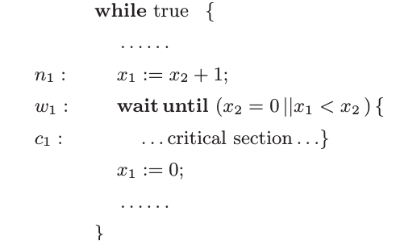
\includegraphics[width = \textwidth]{./images/bakery1.png}
					\caption{variable x represents the ticket}
				\end{figure}
				Then, we need the bisimulation relation. We can express it this way:
				\begin{equation}
					AP = 
					\begin{cases}
						n_i, w_i, c_i \,\vert\, i = 1, 2 \text{ label of the state, two of them}\\
						x_1 > x_2 > 0\\
						x_2 > x_1 > 0\\
						x_2 = 0\\
						x_1 = 0
					\end{cases}
				\end{equation}
				this atomic proposition defines a relation on the states of the composition between the two processes and obtain
				\begin{figure}[H]
					\centering
					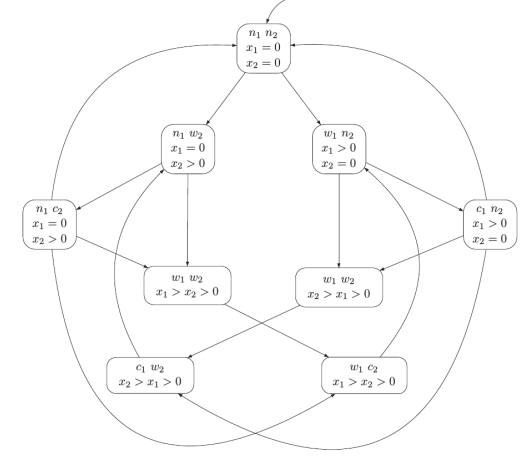
\includegraphics[width = \textwidth]{./images/bakery2.png}
				\end{figure}
				
			
			
			
		
		
		
		
		
		
		
		
		
\end{document}
